\chapter{Introduction}

\section{Overview}
\label{overview}

The ``Rapidly Reconfigurable Research Cockpit'' (R3C) is an innovative design tool for human-systems integration and testing of next generation spacecraft or aircraft cockpits.
The overall objective is to provide an unprecedented ability to optimize a new spacecraft cockpit layout via rapid, low-cost design iterations by integrating state-of-the-art technologies in virtual reality, hand tracking and 3D printing.
The work presented in this dissertation reports on the design and integration of the R3C prototype, as well as a number of experimental results to understand how humans perform in the virtual environment of the prototype, and an evaluation of the performance of the prototype as a design tool.

The motivation for the research presented stems from the design of complex human-machine interfaces such as cockpits for spacecraft and high performance aircraft.
A common problem is that the design (or modernization) of a cockpit will go into flight before evaluation pilots are completely satisfied with the design process, due to time and budget concerns.
The remaining deficiencies of the cockpit design are expected to be overcome through additional crew training.
These deficiencies represent a cost in training throughout the lifetime of the vehicle (typically measured in decades), and ``unknown'' deficiencies of the human-machine system are often discovered too late in accident reports.
To address these issues, we have designed and prototyped a virtual environemnt which allows pilot evaluations to occur earlier and more frequently in the design process.
The aim of our virtual environment is to add the immersion and interactivity benefits of a more functional simulator to a non-functioning geometric mockup.
Mockups are typically used in the early stages of a design process, where large scale changes are more frequent and exact sizing of components are not complete.
With this system, an evaluator can wear a head-mounted display while seated in the mockup to provide an immersive visual layer registered with the physical world, while still retaining their ability to touch and feel the cockpit.
The mockup can then be used for more extensive and realistic cockpit evaluations.
This brings the accompanying benefits of a full simulator with the benefits of early stage design mockups: faster and more drastic redesign iterations.

Specifically, the R3C combines the traditionally separate roles of mockup and simulator.
To achieve this, we use an immersive head mounted display that provides a high fidelity and dynamic view of the cockpit panel, interior, and exterior window views.
The head mounted display is tracked and registered, enabling the cockpit visuals to be overlaid on the low fidelity physical mockup.
The motion and gestures of the cockpit evaluator are tracked using new hand tracker technologies to provide control inputs on the non-functioning cockpit panels.
The low fidelity physical mockup will have a rapidly evolvable cockpit layout with 3-D printed cockpit elements, while still providing an accurate tactile feel.

Human-Systems Integration principles are not sufficiently advanced to reliably design the layout of next generation cockpits without testing.
Thus any new flight deck must undergo crew evaluation and acceptance testing of panel/cockpit human-interface designs.
These evaluations generally result in lengthy and expensive re-design and re-testing cycles.
As a result, a non-optimum design is often accepted in the face of cost and schedule pressures.
In addition, the human factors evaluations are generally done in non-functioning static mockups, which call into question the fidelity of the final, evolved design.

Although many design standards exist for aerospace crew-systems interface design, they mostly serve to guide the technical requirements of the displays, controls, etc. \citep{nasa_human_2010,nasa_nasa_2015,us_department_of_defense_department_1999}.
The cockpit layout and design choices are guided by mission parameters and crew input from mockups \citep{sexton_cockpitcrew_1988,jacobsen_crew_2010,zea_development_2012}.
The importance of the iterative process has been highlighted in many design approaches.
For example, quoting from \citet{nasa_nasa_2015}:
\begin{displayquote}
Human-centered design \textelp is characterized by early and frequent user involvement, performance assessment, and an iterative design-test-redesign process.
\end{displayquote}
Our work does not aim to supersede any existing process or design philosophy, but rather provides a generic tool that all human systems integration engineers can use to enhance their process.
Specifically, we aim to improve the iterative process by reducing cost and time for the redesign cycles.

Another goal of the R3C system is to not only increase the number of iterations, but to improve the feedback from the evaluations.
The use of a mockup for design evaluation is standard in the industry.
\citet{zea_development_2012} reported on design of a cockpit architecture for the then in-development DreamChaser spacecraft.
Three mockup versions were constructed and they found ``a significant amount of knowledge acquired from the mockups was not attainable through computer models''.
A physical mockup that also acts as a simulator will help to improve the feedback of the cockpit evaluations.
Quoting from \citet{sexton_cockpitcrew_1988}:
\begin{displayquote}
\textins{The test pilots} must consider the design in a mission context, as if they are using the systems while flying -- the more realistic the testing environment, the more meaningful the findings.
\end{displayquote}
By allowing the cockpit evaluators to use the mockup as a functioning simulator, the feedback will be more effective in the context of the mission.
A more optimized cockpit will not only reduce pilot workload and increase safety, but also long term cost savings.
When the human-systems integration is performed poorly, the resulting deficiencies can necessitate additional crew-training over the lifetime of the vehicle \citep{jacobsen_crew_2010}.

The prototype system, called the ``Rapidly Reconfigurable Research Cockpit'', consists of a virtual reality (VR) headset, an optical hand tracking device, and 3D printed cockpit surfaces (Figure \ref{fig:intro_r3c}).
The VR head-mounted display (HMD) provides a virtual-visual view of the cockpit environment.
A challenging aspect of immersive VR simulations, however, is to provide a sense of touch.
%an appropriate tactile feel of the objects being interacted with (in our case, the instruments of a cockpit).
We solve this by using 3D-printed instruments co-located with the virtual environment, a technique commonly called ``passive haptics''.
The instruments remain inert and non-functioning in the real world, but appear fully functional in the virtual world presented to the user.
They can be modelled to the exact shape of a cockpit instrument being designed, and printed within a matter of hours.
Instead of requiring the mockup instruments to have functioning buttons, the input of the pilot is read using the hand tracker to provide the interaction with the cockpit.
The optical based hand tracker measures the real-time position of the pilots' hand which is used to determine if the user is touching a button.
The hand tracker also displays the hand in the virtual world for the user, as the use of an HMD blocks the view of one's own limbs.
Additionally, the use of the hand tracker allows for a more thorough examination of the hand movement of evaluation pilots in a new cockpit design than is typically possible.
%Measurements from the hand tracker are used to display the essential visual feedback of hand position in the virtual world, as normally the use of an HMD blocks the view of one's own body.

\begin{figure}
    \centering
    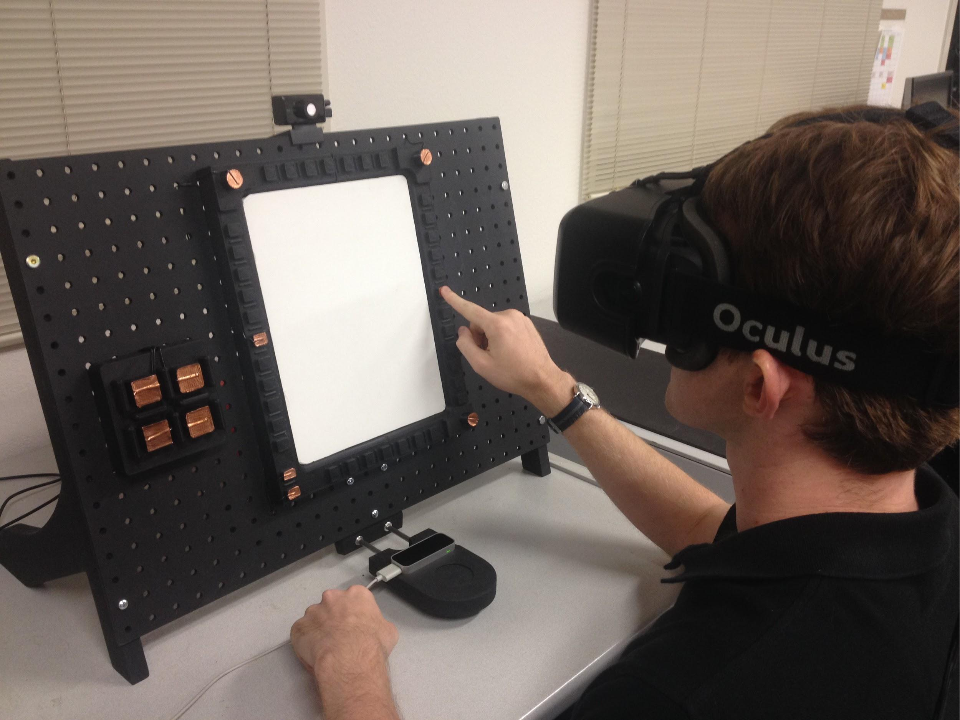
\includegraphics[width=\textwidth]{r3c_no_callout.png}
    \caption{The Rapidly Reconfigurable Research Cockpit prototype.}
    \label{fig:intro_r3c}
\end{figure}

The combination of these technologies allow an existing mockup to be used as a functioning simulator with visuals overlaid on top of screens and/or out-the-window views, and with functioning buttons on the instrument.
With merged mockup and simulator functions, adjustment of the developing flight-deck can be made simpler, cheaper, and more quickly turned around.
The end result of employing this virtually-enhanced mockup/simulator should be a human interface that is truly optimized, which can result in increased flight deck safety and efficiency, as well as reduced crew workload/fatigue.

The R3C prototype has been the technical base for the research performed in this work.
The three main tracks of the research can be summarized in these aims:
\begin{enumerate}
    \item Create a virtual reality system with passive haptics and hand tracking that allows for evaluation of early design cockpits (Chapter \ref{chap:prototype}).
    \item Validate the technical approach and evaluate the performance of subjects in the virtual reality environment with passive haptics (Chapter \ref{chap:pointing} and \ref{chap:ph_exp}).
    \item Evaluate the use of the prototype in a mock design evaluation study to determine the differences in standard performance metrics and subject feedback from using our system (Chapter \ref{chap:de_exp})
\end{enumerate}
The technical approach and development of the prototype is described in Chapter \ref{chap:prototype}.
Three experiments with human subjects have been performed and are reported on to support these aims in Chapters \ref{chap:pointing}, \ref{chap:ph_exp}, \ref{chap:de_exp}.
The first experiment (Chapter \ref{chap:pointing}) asked subjects to repeatedly target one of four buttons on the panel under different conditions, testing differences between real versus virtual world as well as passive haptics versus no passive haptics (mid-air reaching).
We recorded time to completion and accuracy to the button center.
%It was found that the virtual world caused a slight but significant degradation in time for the reaching movement, but no significant change in accuracy.
%The accuracy requirement is more important for our application of safety-critical human-machine interfaces, where accuracy requirements often prevail over movement time.
The second experiment (Chapter \ref{chap:ph_exp}) had subjects perform a Fitts' Law task in different conditions to further characterize the difference between using passive haptics and mid-air reaching.
%The recorded 3D hand trajectory data will also be used to develop the metric for Aim 3 (which is being called the ``task familiarity'' metric or model in this report).
%By using the Fitts' circle for Experiment 2, we can use the Fitts' throughput as a truth measure of familiarity to train and test the model upon.
Additionally, this experiment had a more extensive subject survey to collect the opinions of the subjects, especially their opinion on the differences between passive haptics and mid-air reaching.
The final experiment (Chapter \ref{chap:de_exp}) compared the performance of the R3C prototype as a design evaluation tool against an evaluation using a more traditional simulation.
Subjects were split into two groups, one using the R3C, the other a touchscreen simulator.
Two instrument designs were presented to each subject and they were asked to perform the same task on both.
Afterwards, their comments about the two designs were collected.
Performance measures of the task were also recorded and analyzed.
The goal of the experiment was to determine where subject feedback and performance may differ between an evaluation study using R3C and one using a touchscreen.
The differences found were described and discussed.


\section{Literature Review}
\label{literature-review}

To frame this research, this section will summarize relevant previous work.
The first few sections deal with virtual reality: different haptic environments and evaluation of virtual environments.
Next input device evaluation research such as Fitts' Law is discussed, highlighting work that has been performed evaluations in virtual environments.
%The final section discusses the trajectory models that we propose using as% a basis for extension into a ``task familiarity''
%metric.

\subsection{Virtual Environments for Design}

Recent advancements in virtual reality technology has renewed interest in the benefits of virtual prototyping, and its use has been increasing across industries - manufacturing \citep{choi_virtual_2015}, assembly \citep{pontonnier_designing_2014}, automotive \citep{bordegoni_mixed_2012,lawson_future_2016}, and medicine \citep{nagendran_virtual_2013}.
The term virtual prototyping (VP) is an encompassing term for a variety of virtual interfaces and/or interactions, and any virtual environment can exist on a spectrum from full virtuality to full reality \citep{milgram_taxonomy_1994}.
The use of virtual environments in design processes is well established.
%Virtual manufacturing was described by \citet{shukla_virtual_1994} as ``the use of computer models and simulations of manufacturing processes to aid in the design and production of manufactured products.''
Many design and engineering teams adopted virtual reality early in order to enhance their prototyping process.
\citet{brooks_jr_whats_1999} reviewed the (at the time) current use of virtual reality applications in industry.
A number of engineering design firms had already seen the potential for using virtual whatsity set ups in design reviews, though display applications were typically wall-projections instead of a head mounted display.
John Deere claimed \$80K of savings from preliminary mockup costs from using the VR system and Chrysler performed some ergonomic reviews using a head mounted system, though the HMDs at the time were very heavy and low resolution \citep{brooks_jr_whats_1999}.
\citet{abate_haptic-based_2009} investigated the use of haptic interactions for virtual reality training of assembly and maintenance task, and performed a usability assessment which found technicians preferred the use of haptics in a virtual maintenence task.

Flight simulation was one of the first applications of virtual environments, and the use of virtual environments for training and development of new cockpits has persisted throughout the years \citep{hancock_human_2008}.
Virtual reality simulators for aviation have recently become a track of research.
\citet{wan_mrstudio:_2011} used an augmented reality approach to register a virtual-visual layer on top of a mockup of a commerical aircraft cockpit for design and evaluation.
\citet{yavrucuk_low_2011} combined an immersive head-mounted display with hand tracking gloves to provide a virtual simulator of a helicoptor.
They did not use any haptic feedback and users interacted with the instruments using the hand tracking, with no physical mockup.
\citet{aslandere_virtual_2015} had a similar technical setup and focused on the virtual button interaction.
They found that the collision volume for a virtual button interaction did not impact the interaction, but a more realistic hand avatar increased effeciency.
The first appearance of work similar to ours was by \citet{schiefele_simple_1998} in Germany, which also used a head-mounted display (HMD) to replace the visuals of a flight simulator (though technology has drastically changed in HMD's since their work).
They recreated only the positions of the panels with a flat plate and then used a magnetic hand tracker for reading the pilot input.
A short usability study was presented, and they found that users could activate switches, knobs and dials in less time with the physical panel than without (i.e.\ reaching into mid-air).

\citet{aromaa_suitability_2016} reviewed the use of virtual prototypes for human factors/ergonomics (HFE) evaluation.
They found that the fidelity of a VP may not affect subjective results, but that task performance can be affected, hindering the utility of the evaluation itself.
This is supported by findings that decreased presence (the feeling that the simulation is real) can negatively affect task performance \citep{youngblut_relationship_2003}.
Presence is discussed in more detail in a later section.
\citet{lawson_future_2016} provided recommendations for incorporating VP in the automotive industry for HFE evaluation, including using haptic feedback and marker-less body tracking.
They found that the use of markers can encumber the participant, affecting evaluation results.


\subsection{Virtual Tactile Environments}
\label{virtual-tactile-environments}

One of the challenges of virtual environments has been presenting the user with a tactile sensory input that matches the visual sensory inputs they are experiencing.
Many haptic glove products have been created that attempt to simulate this with motor vibrations.
Since they are attached to your body, they cannot provide any external stopping force, so the simulation can break down when interacting with rigid objects.
Another technique is using a stylus mounted to a 6-DOF actuator that can simulate external forces.
These have been used for many studies with the application of surgical tasks, when a tool would be used in the real scenario as well.
The focus of this work is the idea of \emph{passive haptics}, whereby the tactile environment is recreated to provide the sense of touch, including external forces.
The disadvantage is that the tactile environment cannot dynamically change during the simulation.
Some researchers have attempted to create robotic passive haptics \citep{mcneely_robotic_1993, tachi_construction_1994}, which use a robotic arm to deliver the appropriate tactile experience to the user as they reach into the virtual world.
This approach quickly becomes complicated and expensive.
Others have tried approaches to morph the virtual world to adapt to a generic passive haptic device \citep{kohli_exploiting_2009,kohli_redirected_2012}, which can work only for small discrepancies.
Fortunately, the adaptability during a simulation of the passive haptic environment is not a requirement for the use case of a pilot evaluating a new cockpit interface.
We still retain the ability to quickly change the environment in between simulation sessions via 3D printing new parts.

Previous work with passive haptics, though limited, have shown it to provide benefits.
\citet{insko_passive_2001} investigated the impact of passive haptics on generic virtual environments.
It was found that the passive haptics increased the sense of presence felt by users.
An experiment had two groups complete a maze in a virtual environment, one group with passive haptics on boundaries, and one without.
After training the passive haptic group bumped into far fewer obstacles than the group without.

\citet{borst_evaluation_2005} created a ``mixed'' haptic virtual environment, whereby they combined an active haptic glove with a passive haptic panel.
The panel provided the stopping force and depth location of the interface, while the glove haptics provided the finer details of the buttons, switches and dials.
They compared subjects performing tasks on the panel using the glove by itself (no panel), the passive haptics by itself, as well as their mixed condition.
They found the glove by itself consistently performed worse than the other two, but overall no significant difference existed between passive haptics and their mixed haptics.

\subsection{Virtual Environment Evaluation}
\label{virtual-environment-evaluation}

It is notoriously hard to quantify the effectiveness of a virtual environment (VE).
One can report on quantitative measures of the virtual reality (VR) setup such as latency, field of view, resolution and others, but in the end the only useful measure is whether the user finds the virtual environment convincing.
This can also change depending on the user -- one user could find a VE convincing while another finds it intolerable.
The effectiveness of a VE is often linked to the sense of \emph{presence}, defined ``as the subjective experience of being in one place or environment, even when one is physically situated in another''\citep{witmer_measuring_1998}.
\citet{sheridan_musings_1992} argued that presence is a subjective sensation that necessitates a subjective measure.
Two of the more popular post-questionnaires that have been developed are the Presence Questionnaire (PQ) \citep{witmer_measuring_1998} and the Slater-Usoh-Steed (SUS) questionnaire \citep{slater_depth_1994}.
The former (PQ) consists of 32 questions that cover various factors of presence such as sensory, control, distraction and realism.
The SUS questionnaire consists of only 6 questions and is focused on the feeling of presence.
\citet{nystad_comparison_2004} found the PQ to be more sensitive to technology and interaction methods, while the SUS fits better to the definition of presence.
This suggests PQ may be better suited for our work when comparing between conditions, but SUS could be useful as a general evaluation of the overall system.
The increased presence with passive haptics found by \citet{insko_passive_2001} is an important finding we aim to replicate for our virtual environment.

Presence is an important measure as it has been shown to correlate with performance in the virtual environment \citep{youngblut_relationship_2003}.
A high sense of presence increases the feeling that the objects shown in the virtual environment are real and the interactions are the same as they would be in the real world.
It also provides the user with a better memory of the environment \citep{dinh_evaluating_1999}.

We also hypothesize that our system will reduce the amount of arm fatigue experienced by the operator compared to a mid-air pointing virtual environment (i.e.\ no tactile workstation present).
This common phenomenon in virtual environments is often called gorilla arms, as people feel that their arms are too heavy to support after prolonged use reaching out into the void.
A measure of this arm fatigue is not included in the standard presence questionnaire.
The literature does not contain a large volume of experiments that measure arm fatigue.
Qualitative measures include the Likert scale, NASA Task Load Index (NASA TLX), the ISO-9241-9 ``Assessment of Comfort and Fatigue'' and the Borg scales (RPE and CR10).
The Borg CR10 performs favorably to the other scales for measures of exertion \citep{grant_comparison_1999}.
Recently, a quantitative approach has been proposed that uses optical tracking of the arm and wrist which validated well against a Borg CR10 scale \citep{hincapie-ramos_consumed_2014}.
Adapting their software to our system would be out of scope (and requires more upper-limb measurement than we are currently capable of) but the validation against the Borg CR10 scale is promising.

\subsection{Workload}

\tinytodo{working on this...}
Workload is a term used to describe the amount of work an individual has to do.
For aviation and space cockpit design, managing the amount of workload of the pilot is paramount.
``construct that represents the cost incurred by a human operator to achieve a particular level of performance''.
It is an important measure of a design evaluation study of any cockpit.
It can be measured many ways.
In this work, NASA-TLX is used as it is the most used.

\subsection{Input Device Evaluation}
\label{input-device-evaluation}

For decades one of the most important empirical models in the Human-Computer Interface (HCI) community has been Fitts' Law.
The basis of the model is a method to predict the movement time of a user towards a target.
Using just the size and distance to the target, the average movement time can be accurately predicted after emperically determining the model parameters.
It has been used to evaluate new input devices to determine how fast a user can move to a target (e.g.\ mice, trackballs, joysticks), as well as a guideline for interface designs (ensuring that target areas are the right size).
A summary of the field is presented here, with notable contributions and similar work following.
Fitts' Law used in the context of virtual environments and our work is then discussed.

\subsubsection{Fitts' Law}
\label{fitts-law}

\citet{fitts_information_1954} originally reported on his experiments of targeted reaching movements between varying target sizes, and compared the linear trend he discovered to information theory models.
He postulated that the entire control system of the human, from motor control to visual and proprioceptive feedback, can process information at a certain maximum rate, and the bandwidth of the channel must be derivable from the physical parameters of the target.
Fitts' adapted Shannons' Theorem \citep{shannon_communication_1949} from information theory for the bandwidth of a channel in the presence of a signal and noise.
The distance to the target (\emph{D}) is considered the signal, and the width of the target (\emph{W}) is considered to be the noise (Figure \ref{fig:intro_fitts}).
This analogy allowed Fitts' to create a formula for the \emph{index of difficulty} (\(\text{ID}\)) of a target:

\begin{equation}
    \mathrm{ID} = \log\left(\frac{2D}{W}\right)
    \label{eq:intro_id}
\end{equation}

It was found experimentally that the index of difficulty is linearly correlated to \emph{movement time} (MT), the time taken to move between the start and the target.
This leads to the equation that is now known as Fitts' Law:

\begin{equation}
    \mathrm{MT} = a + b \cdot \mathrm{ID}
\end{equation}
where \emph{a} and \emph{b} are the parameters of the linear regression, which are determined experimentally.
A typical experiment consists of subjects performing movements to a range of targets with varying index of difficulty, and recording their movement time.
The data is then fit to a linear regression.

\begin{figure}
    \centering
    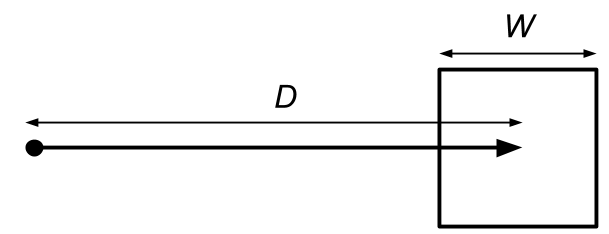
\includegraphics[width=0.5\textwidth]{fitts_dimensions.png}
    \caption{The dimensions of a Fitts' Task (\emph{D} = distance, \emph{W} = width)}
    \label{fig:intro_fitts}
\end{figure}

Since its original formulation, refinements to the model have focused on the formula for index of difficulty, \(\text{ID}\), and the definition of its dependencies, width and distance.
\citet{crossman_speed_1957} suggested a very important refinement called the adjustment for accuracy.
This provides a correction to the \(\text{ID}\) to compensate for the task which is actually performed by the subject as opposed to the task that was asked to be performed.
For example, if a subject is presented with two large targets close together ($D << W$), then he/she tends to aim towards the inner edges of the targets instead of the center, effectively using a much smaller target width.
The adjustment for accuracy replaces the width, \(W\), with the \emph{effective width}, \(W_{e}\).
The basis for this adjustment is that the information theory basis for Fitts' Law expects that the ``noise'' of the target width induces a 4\% error rate \citep{mackenzie_fitts_1992}.
If more or less than 96\% of the target hits are successfully within the target, then the target width is adjusted with the adjustment for accuracy to fit the target error rate of 4\%.
Motor tasks have been shown to be a Gaussian distribution \citep{crossman_feedback_1983,woodworth_accuracy_1899}, thus 96\% of target endpoints will be within 4.133 standard deviations (\(\sigma\)).

\begin{equation}
W_{e} = 4.133\sigma
\end{equation}

It is recommended to calculate the effective width for each subject in each condition as it is sensitive to both between and within subject variability.
The effective width can then be used to calculate an \emph{effective index of difficulty}, \(\text{ID}_{e}\).
The effective width described here is for one dimensional targets, but there are extensions to 2D targets as well \citep{murata_extending_2001}.

The form of the logarithmic term in the index of difficulty equation (Eq.\ \ref{eq:intro_id}) has encountered some debate over the years.
Fitts did not describe the reasoning for including the factor of two in his original formulation, and \citet{welford_fundamentals_1968} suggested a modification that provided a better fit for low values of index of difficulty.
The Welford modification simply adds
\begin{equation}
    \mathrm{ID} = \left( \frac{D}{W} + 0.5 \right).
\end{equation}
A more recent variation noted by \citet{mackenzie_note_1989} suggests that by comparing to Shannons' Theorem, as Fitts originally proposed as the theoritical basis for his work, then the form should be,
\begin{equation}
    \mathrm{ID} = \left( \frac{D + W}{W} \right) = \left( \frac{D}{W} + 1 \right)
\end{equation}
which has been widely adopted in literature as the Shannon's Formulation.
The mathematical structure of this formulation, unlike the original equation, will not produce a negative index of difficulty with real, positive dimensions.


The first use of Fitts' Law in the human-computer interface (HCI) community was with \citet{card_evaluation_1978}, comparing the use of a mouse, joystick and keys for text selection.
This led to an extensive use of Fitts' Law in the HCI field, both as a way to evaluate input devices and a design law for user interfaces.

Best practices of using Fitts' Law have been developed, and the standard ISO-9241-9:2000 provided guidelines for the use of Fitts' Law in evaluation of input devices\citep{international_organization_for_standardization_iso_2000}.
Most notably, it was suggested to use the ISO-9241 ``Fitts' circle'' for evaluations of 2D tasks (Figure \ref{fig:intro_fitts_circle}).
This input pattern has been adopted widely in literature, and provides a standard for comparing across studies.

\begin{figure}
    \centering
    
\includegraphics[width=0.5\textwidth]{fitts_circle.png}
    \caption{ISO-9241 Fitts' Circle or multidirectional tapping task.}
    \label{fig:intro_fitts_circle}
\end{figure}

\citet{soukoreff_towards_2004} present a review of the best practices for designing and performing a Fitts' law experiment, including the use of the Shannon Formulation and the ISO-9241 ``Fitts' circle''.
They also advise the use a large range of ID values, ideally from 2 to 8 bits.

%Many experiments achieve this by varying distance and width, but Guiard (2009) points out the inconsistency of designing for a range of ID based on two factors, and shows that by holding one fixed lowers the regression error, while reducing experiment complexity.
%Wobbrock (2011) provided an independent validation of this, showing that significant effects remained when retroactively removing the varying diameter of targets.

When used to evaluate input devices, the metric of comparison is often \emph{throughput}.
Throughput (TP) is defined as the index of difficulty (ID) over the movement time (MT).
\begin{equation}
    \mathrm{TP} = \frac{\text{ID}}{\text{MT}}
\end{equation}
The units of throughput are bits per second, and it represents the information capacity of the input device.
A higher throughput indicates that the human is able to convey more information (\emph{bits}) through one input device versus another in a given time (\emph{per second}).
\citet{soukoreff_towards_2004} recommend the use of throughput as the measure for comparing experimental conditions as well.
One of the advantages of using throughput is that it combines speed and accuracy requirements through the use of the index of difficulty.
Throughput has been validated to be invariant to subjects prioritizing speed or accuracy \citep{mackenzie_fitts_2008}.

The debate on which form and refinement of Fitts' Law is the best to use continues to this day \citep{drewes_only_2010,hoffmann_which_2013}, and this work will not attempt to settle this debate.
%\tinytodo{rewrite this}However, the understanding of the origin of Fitts' Law, best practices and the many forms of the equations will greatly influence the design and success of the experiments performed.
Since no form of the equations have been rejected outright in the literature, it is recommended to perform analysis with all versions and note if any significant differences in major conclusions result \citep{soukoreff_towards_2004}.

\subsubsection{Dimensionality of Fitts' Law}\label{dimensionality-of-fitts-law}

Throughout the Fitts' Law literature one of the differences between experiments is how many dimensions the subjects can move (or move their cursor).
There are two dimensionalities to consider when discussing Fitts' Law experiments: the dimensionality of the targets or task, and the dimensionality of the movement.
A 1D task means the targets are aligned along a single axis, whereas a 2D task has them located on a plane (such as the Fitts' circle in Figure \ref{fig:intro_fitts_circle}).
The dimensionality of the movement refers to how many dimensions the subjects need to move when moving between the targets.
For example, the original Fitts' Law task was a 1D task as the targets were varied in width along the movement direction, but sufficiently long in the perpindicular dimension, removing that dimension as a variable.
The movement however was effectively 2D, as the subjects could (and needed to) lift up from the table to move between targets.

The popularity of Fitts' Law in the HCI field has led many researchers to focus on the use of Fitts' Law on a 2D computer screen controlled by a mouse.
This is a 2D task, with a constrained 2D movement.
For our application, the movement we are insterested in is a 2D task with 3D movement since the buttons on a cockpit panel are configured in approximately a single plane, with pilots reaching towards them in uncontrained 3D movement.
There are some newer HCI studies that present this task and movement dimensionality, as it is analogous to the use of a touchscreen device.
Some have proposed minor variations to the formulation of Fitts' law to adjust for touchscreens \citep{bi_ffitts_2013,sears_high_1991}, but others have found the original formulation to perform well \citep{mackenzie_fitts_2015}.
There are also studies discussed in the next section that perform this task in a virtual environment.

Refinements have been proposed to account for the possible effects of extending the task dimensionality to 2D, such as the bivariate target model \citep{accot_refining_2003, mackenzie_extending_1992, wobbrock_error_2008}.
Some work has also explored this for 3D tasks, introducing a trivariate model \citep{grossman_pointing_2004} and corrections for 3D placement of targets \citep{cha_extended_2013, murata_extending_2001}.
These experiments place targets in a truly 3D space, with of course 3D motion required of the user.
The use of a Fitts' circle on the 2D plane removes the need for these accomodations, as the targets are symmetric and have the same width when approached from any direction.

\subsubsection{Fitts' Law in Virtual Environments}\label{applying-fitts-to-virtual-environment}

Fitts' Law has been used in evaluating virtual environments and their input devices.
\citet{chun_evaluating_2004} evaluated a set of 3D stereo displays with a single haptic-enabled stylus using a Fitts' tapping task.
They did not have well-fit regressions, but this could have been due to a small range of ID values used (2-3), targets being placed in 3D space (a 3D task with 3D movement) with random order (making the sequence of the task unlearnable), and averaging across subjects before completing the regression.
\citet{teather_evaluating_2010} performed a similar task and also found an underperformance of the regression in the fully 3D task.
One condition performed a mid-air 2D planar task with 3D movement, and no significant difference in throughput was found compared to the same task with constrained 2D motion.
\citet{liu_comparing_2009} performed a planar multi-directional Fitts' task with a stereoscopic display, and compared virtual world to real world results, finding movement time twice as long in the virtual condition.
The trajectories were analyzed to determine where the extra movement time was spent, which is discussed in the next section (\nameref{human-targeting-motion}).

One of the few experiments that utilize Fitts' Law in an immersive HMD was performed by \citet{kohli_redirected_2012} who were focused on evaluating discrepant (warped virtual space) virtual environments to fool the user of the nature of the physical world.
They had the subjects perform an ISO-9241 Fitts' circle on a panel placed in front of them, and in some conditions the panel was rotated in the virtual world but not in the real world to create the discrepancy.
The subjects' hand movement was warped to compensate for this.

\citet{coelho_pointing_2014} evaluated the LeapMotion hand tracker (the same technology we are using) in a 3D Fitts' task (with visual feedback on a computer screen), but did not perform a Fitts' model analysis, comparing only time.
\citet{seixas_one_2015} performed an ISO 9241-9 Fitts' circle task with the LeapMotion.
Their goal was to compare a gesture based selection technique, and they provide a Fitts' throughput comparison between that and direct mid-air selection.

\subsection{Human Targeting Motion}
\label{human-targeting-motion}
%
%\subsubsection{Trajectory Models}\label{trajectory-models}
%
Fitts' Law provides a validated model for predicting movement time of a human movement, but this only provides part of the story.
Analyzing overall time of movement simplifies the complex trajectory that a human forms in their movement, but it leaves us with only one measure of performance.
With the use of the hand tracker we can quantify a complete 4D dataset of the reaching movement -- 3D position and time.
This allows us to unobtrusively investigate a more complete picture of the motion of the subject than has been technologically possible until the last few years.
The trajectory of a human arm motion in a point-to-point multi-joint arm movement can take an infinite number of paths due to the complex joint structure of the human arm.
It has been observed in many experiments, however, that humans tend to follow a common trajectory -- a roughly straight spatial path, with a bell-shaped velocity profile.
%This observation has led researchers to create mathematical models to predict the trajectory.
%
%The \emph{minimum jerk} model was first proposed by Flash \& Hogan (1985), and provided very good agreement to experimental data.
%Their hypothesis for the model is that the human hand trajectory in point-to-point movements follows the trajectory that supplies the minimum amount of jerk (time derivative of acceleration).
%This provides a simple optimization criterion,
%
%%\begin{longtable}[c]{@{}lll@{}}
%%\toprule
%%&
%%\(C_{J} = \frac{1}{2}\int_{0}^{t_{f}}{\left( \frac{d^{3}x}{dt^{3}} + \frac{d^{3}y}{dt^{3}} + \frac{d^{3}z}{dt^{3}} \right)^{2}\text{dt}\ }\)
%%& \protect\hypertarget{ux5fRef319839852}{}{}Eq. 2\tabularnewline
%%\midrule
%%\endhead
%%\bottomrule
%%\end{longtable}
%
%where the \(x\), \(y\), and \(z\) are the position coordinates, and the integral covers the time period of interest, \(t\).
%The model has remained popular due to its simplicity, and ability to provide a closed form solution.
%It is a purely kinematic model, meaning that it does not require any knowledge of the human arm itself.
%The model can be solved for an optimized trajectory with only the initial and final conditions.
% If Eq.
%2 is solved with initial and final conditions of zero velocity and acceleration, then this provides a closed form and decoupled solution, presented here for \(x\), but \(y\) and \(z\) take the same form:
%
%%\begin{longtable}[c]{@{}lll@{}}
%%\toprule
%%&
%%\(x\left( t \right) = \ x_{0} + \left( x_{0} - x_{t} \right)\left\lbrack 15\left( \frac{t}{t_{f}} \right)^{4} - 6\left( \frac{t}{t_{f}} \right)^{5} - 10\left( \frac{t}{t_{f}} \right)^{3} \right\rbrack\)
%%& \protect\hypertarget{ux5fRef319840064}{}{}Eq. 3\tabularnewline
%%\midrule
%%\endhead
%%\bottomrule
%%\end{longtable}
%
%where \(x_{0}\) and \(x_{f}\) are initial and final position, respectively, and \(t_{f}\) is the time of the movement.
%A plot of the solution of Eq.
%3 for position and velocity is shown in Figure 5.
%
%The minimum jerk model performs well for many trajectories, however since it relies only on the kinematic variables, it does not take into account arm length, external force or load, or range of motions.
%Uno et al.
%(1989) proposed his \emph{minimum torque} model based on the theory that humans must plan their movement based on a physical variable, and found that minimizing torque at each joint provided a good fit to experiment.
%The minimum torque model was refined to the minimum torque-change and renamed the \emph{minimum commanded torque} model (Nakano et al., 1999), and the optimization criterion is presented here.
%
%\[C_{T} = \frac{1}{2}\int_{0}^{t_{f}}{\sum_{i = 1}^{N}{\left( \frac{d\tau_{i}}{\text{dt}} \right)^{2}\text{dt}}}\]
%
%where \(\tau_{i}\) is the torque at the \emph{i}-th joint.
%\emph{N} is the number of joints and \emph{t} the time of the movement.
%Since jerk is dependent on torque, it is not surprising that the trajectories predicted using this model are quite similar to those of the minimum jerk model (Breteler, Meulenbroek, \& Gielen, 2002).
%The differences are that due to the modeling of the kinematics of the arm the minimum torque-change model predicts curvature in the trajectory positional data (Figure 6).
%As shown in Figure 5, the minimum jerk predicts a symmetric velocity profile, scaled by time and distance.
%Several experiments have shown that the deceleration phase (time from peak velocity to target) is longer than the acceleration phase (time to peak velocity) (C.
%L.
% MacKenzie, Marteniuk, Dugas, Liske, \& Eickmeier, 1987; Milner, 1992; Uno et al., 1989).
%The minimum torque-change model more accurately depicts this velocity asymmetry.
%

%\subsubsection{Adaption to Novel Dynamics/Environments}\label{adaption-to-novel-dynamicsenvironments}
%
%One of the assumptions of the minimum jerk and torque models is that the subject is performing rapid aimed movements (i.e.
%well trained and no cognitive workload), much like the requirement of Fitts' Law.
%This implies that the trajectories do not match the model as well when the subject is learning the pattern of movement, or introduced to a novel situation.
%Most articles do not report on the learning phase and report data after training effects have worn off.
%The learning phase is something we are interesting in characterizing for the development of our trajectory based training level model.
%There are a few studies that have investigated the adaptation of subjects to novel dynamics, by adding artificial forces to an end effector that is moved by the subject (Conditt, Gandolfo, \& Mussa-Ivaldi, 1997; Scheidt, Reinkensmeyer, Conditt, Rymer, \& Mussa-Ivaldi, 2000).
%These show that subjects initially experience deviations from the minimum torque model, but will approach the optimal movement over a number of trials.
%
%\subsubsection{Trajectories in Virtual Environments}\label{trajectories-in-virtual-environments}
%
In one of the earliest experiments to measure trajectories of human targeting motions, \citet{woodworth_accuracy_1899} discovered that there are two distinct phases of the targeting motion: a ballistic phase and a corrective phase.
Subjects typically perform the bulk of their movement in the ballistic phase, often considered more of an open-loop or feed-forward mechanism, and as they near the target switch to a feedback, closed-loop, corrective phase \citep{elliott_control_1999}.

Experiments in virtual environments have shown that users typically spend more time in the corrective movement phase than when performing the same task in a non-virtual environment \citep{liu_comparing_2009}.
However, this work was completed for a mid-air interaction, so it is an open question whether the introduction of passive haptics would reduce the corrective phase penalty for operating in a virtual environment.
We can quantitatively investigate this question with the use of our virtual environment.
\citet{mackenzie_three-dimensional_1987} showed that there was correlation between the target size and the time of the deceleration phase for a Fitts' task, suggesting that subjects will adapt their trajectory for accuracy requirements.
Our application to a cockpit environment is one where accuracy demands are often more important than time demands for manipulation of instruments.
%
%\subsubsection{Other Trajectory Metrics}\label{other-trajectory-metrics}
%
Other metrics have been developed in the literature to evaluate the trajectory of a targeting motion.
\citet{meyer_optimality_1988} developed a parsing criterion to divide the trajectory into submovements and defined three types: return from overshoot, accelerate due to undershoot, and slowing towards target.
\citet{mackenzie_accuracy_2001} presented a set of accuracy measures for targeting motions based on trajectory information.
They were developed to compliment a Fitts' input device evaluation.
The measures are named target re-entry, task axis crossing, movement direction change, orthogonal direction change, movement variability, movement error, and movement offset.
They quantify types of movement that are not along the ideal straight-line path from start to goal.

\subsection{Summary}
\label{summary}

The combination of immersive virtual reality simulator with an inert passive haptic has not been extensively tested in the virtual reality literature.
Other approaches at immersive haptics have focused on creating a dynamic environment, but our application of a static cockpit does not need to change geometrically during the simulation (not to be confused with our re-configurability between simulations).
The integration of new hand tracking technologies is a further innovation, allowing us to provide interactivity with the passive haptics.

To evaluate this new virtual environment, we aim to use two validated measures -- presence and Fitts' Law.
Fitts' Law is a well validated and actively used model for evaluating both input devices and interfaces.
To date there have been only a few uses of Fitts' Law in immersive head-mounted display virtual environments.
As of our knowledge, no one has performed a Fitts' Law experiment in a virtual environment using the new generation optical hand trackers (i.e.\ the LeapMotion we are using).
A Fitts' Law characterization is an important step to take to evaluate the system we have created, and provides a standard means of comparison across previous and future literature.

\tinytodo{paragraph summary for de experiment}

\section{Research Questions}
\label{hypotheses}

The research presented in this work consists of three experiments with human subjects to answer our fundamental research questions.
As is natural with research work, our research questions and motivations evolved with the findings of the previous experiment.
Presented here are a summary of the major research questions that were investigated with the experimental work.
The questions are further detailed in their respective experiment chapters.

\begin{itemize}
    \item Can the technical approach of a mockup providing passive haptics with a visual-virtual overlay using a head mounted display be used successfully?
    \item Can a user select a button in the R3C prototype with the passive haptics and hand tracker as accurately as one in the real world?
    \item Does the use of passive haptics change the performance of a subject targetting a button in the virtual environment?
    \item Does the use of passive haptics increase the presence of subjects using the virtual environment?
    \item Can the R3C prototype be used effectively as a design evaluation tool?
    \item How does the R3C prototype compare to other design evaluation tools?
\end{itemize}

\tinytodo{summary of lit review and upcoming work}

%\section{Experimental Methods}
%\label{experimental-methods}
%
%The experimental work is to be segmented into three major experiments.  The experiments build on the knowledge of the previous, but some of their goals are overlapping.
%
%\begin{enumerate}
%\def\labelenumi{\arabic{enumi}.}
%\item Reaching task to evaluate virtual environment and input methods
%\item Fitts' circle evaluation of virtual environment and input methods, development of task familiarity model
%\item Validation of task familiarity model through a representative pilot task
%\end{enumerate}
%
%Experiment 1 has been completed, and the results will be presented here.  Experiment 2 is planned and outlined here. The second experiment builds on what we learned in the first experiment for evaluating the technology, and the data analysis will begin the development of the task familiarity model. The plan of Experiment 3 is to further develop and validate the model, and so it will depend on the results and lessons learned from Experiment 2. A candidate experimental design is presented within.
%
%\subsubsection{Experiment 1}\label{experiment-1}
%
%The first experiment was designed to evaluate our technical approach and measure some aspects of performance between experimental conditions. A brief description and summary of the results are given here, but a more thorough treatment is given in Joyce \& Robinson (2015). There were three main effects of the targeting task under study in this experiment:
%
%\begin{itemize}
%\item
%  The effect of the use of the Virtual Reality (VR) head-mounted display
%  (HMD) versus no VR HMD (i.e. virtual vs. real world).
%\item
%  The effect of the physical panel versus no physical panel present
%  (i.e. having the tactile feedback vs. no tactile feedback).
%\item
%  The effect of the optical tracking button detection versus the
%  capacitive touch button detection.
%\end{itemize}
%
%The capacitive touch sensors mentioned in the last effect were custom
%developed capacitive sensors mounted on top of the buttons that
%registered a finger touching them, as well as position of the finger on
%the button within 0.08in. We developed this technology in order to
%provide a reliable ``truth sensor'' for button press detection to
%compare our optical tracking against, and for comparing accuracy between
%conditions.
%
%Figure 7 shows a diagram of the experimental setup. Figure 8 shows a
%photo of the experiment with a view of the virtual world as well. The
%panel was configured with a single four-button keypad (``Button Pad'' in
%figure). Three different ``Start Pads'' were placed on the edge of the
%desk near the subject. The participants were asked to start with their
%index finger on one of the three ``Start Pads'' and then target the
%correct button on the ``Button Pad'' panel. Audio prompts were given
%through headphones that indicated the starting pad and panel button goal
%before each task. Subjects were instructed to target the center of the
%correct button, but were given no instructions on speed. Eight (8)
%subjects performed 48 targeting tasks after 12 training trials under
%each of the following four (4) different conditions:
%
%\begin{enumerate}
%\def\labelenumi{\arabic{enumi}.}
%\item
%  Wearing the HMD (head mounted display), button selection registered by
%  capacitive sensors, panel physically present
%\item
%  Wearing the HMD, button selection registered by hand tracking sensors,
%  panel physically present
%\item
%  Wearing the HMD, button selection registered by hand tracking sensors,
%  panel not physically present
%\item
%  Not wearing the HMD, button selection registered by capacitive
%  sensors, panel physically present
%\end{enumerate}
%
%The dependent variables measured were:
%
%\begin{itemize}
%\item
%  time from starting pad to trial goal button
%\item
%  accuracy measured on the capacitive touch sensors (for panel present
%  conditions)
%\item
%  success rate (selected correct button within 10 second time limit)
%\end{itemize}
%
%Due to the difference in distance between the three different start pads
%and four goal buttons, the time recorded was scaled by the total
%movement distance over the average movement distance, which is reported
%here as ``corrected time''. Table 1 summarizes the results, and Figure 9
%illustrates the effects being investigated. The significances of the
%effects of were determined using a two-sample t-test on the corrected
%time measure between the appropriate conditions (e.g. effect of use of
%head mounted display compares condition 1 and 4, which both use
%capacitive sensors and panel present). The effect of the use of the HMD
%was significant (p~\textless{}~0.01), and on average caused the
%corrected time to decrease from 1.88 seconds to 0.59~seconds. The
%optical detection algorithm also caused a significant (p \textless{}
%0.01) decrease on corrected time compared to the capacitive sensors,
%from 2.43 seconds to 1.88 seconds. The panel versus no panel test found
%no significant effect on time. The selection of the correct button was
%performed almost without error, which is a promising result for new
%users of the system. There was no significant effect between the
%different conditions on success rate. Over 8 subjects and 1517 trials,
%only 12 trials selected the wrong button and only 12 trials timed out,
%giving an overall 98.4\% success rate. Observations made during the
%experiment indicate that at least some of the wrong button selections
%were due to misheard prompts or loss of attention. The accuracy of the
%button press itself was also measured by recording location of the
%finger while on the capacitive touch pad. The distance from button
%center results showed no significant change between the virtual world
%conditions, with only 0.10 inches difference between real world and
%virtual world accuracy. Due to the accuracy of the sensor (0.08~inches
%in each axis), this is not a significant change.
%
%The results indicated that there was a performance decrement in terms of
%time in the virtual environment compared to the real world. This is
%consistent with previous work, though our pilot studies indicate this
%could be reduced for trained subjects. We found no effect in time to
%button between the tactile environment and the mid-air environment,
%however subjective results on presence were inconclusive. The
%questionnaires were given after the subject completed the entire
%experiment, so a full presence measure could not be given for each
%condition. The sense of presence for each condition is important for us
%to try to measure conclusively in Experiment 2.
%
%\subsubsection{Experiment 2}\label{experiment-2}
%
%The goal of the second experiment is to further investigate the effect
%of the panel in the virtual environment. The results of the first
%experiment indicated that reaching time was not affected if the panel
%was present, but we hypothesize there are other effects we have not
%measured. The goals of the experiment are:
%
%\begin{itemize}
%\item
%  Quantify the Fitts' throughput between with passive haptics (with
%  panel) and without passive haptics (no panel, mid-air reaching)
%\item
%  Assess the subjects' reporting of presence and arm fatigue in virtual
%  world between passive haptics and no passive haptics
%\item
%  Measure and perform analysis on the button-to-button 3D hand
%  trajectories of the subjects
%\end{itemize}
%
%Subjects will be seated in front of the panel similar to the setup in
%the first experiment, and perform the task in two conditions. The task
%will be a Fitts' ISO-9241 circle sequence (see section Fitts' Law,
%Figure 4). The subjects will perform the Fitts' circle sequence for a
%range of indices of difficulties (3.45 to 5.36 bits), corresponding to
%diameters (\emph{D}) of 20cm, 30cm and 40cm and button diameters
%(\emph{W}) from 10mm to 30mm in 5mm increments. The button diameter
%ranges are chosen based on MILSPEC ranges for cockpit buttons (US
%Department of Defense, 1999). For each condition, the subjects will
%complete a set of blocks of Fitts circles, where one block is a sequence
%of one sized circle. The two experimental conditions will be:
%
%\begin{itemize}
%\item
%  In virtual environment, panel in position providing passive haptics
%\item
%  In virtual environment, no physical panel (mid-air reaching)
%\end{itemize}
%
%Every subject will perform both conditions, which will be presented to
%the subjects in alternating order. We are aiming to recruit 10-20
%subjects who have little or no prior virtual reality experience. After
%performing each condition the subjects will complete a ``presence''
%questionnaire to evaluate if the physical panel provides a higher level
%of presence. The questionnaire will also inquire about the subject's
%self reported arm fatigue, as this is a major problem with mid-air
%pointing in virtual environments.
%
%The use of the standard Fitts' circle will allow us to compare the
%throughput to other experiments, most notably we would expect a similar
%throughput to the experiment performed by Kohli et al. (2012) in their
%baseline condition for the passive haptic condition, and a similar
%throughput to Seixas et al. (2015) for the mid-air condition.
%
%It has been shown in many experiments that the Fitts' throughput will
%asymptotically approach the final value as the subject learns the input
%device and task. Typically, this behavior is only used to determine
%which trials to include in the Fitts' regression -- only trials with
%trained behavior are used to satisfy the ``rapid-aimed movements''
%requirement of Fitts' Law. For our data analysis, these ``training
%trials'' will be used to develop the ``task familiarity'' trajectory
%metric. We hypothesize that when the subject is learning the task (and
%the virtual environment) they will move between buttons in a less
%energy-optimized trajectory than when they are fully trained. The
%minimum jerk model describes an experimentally validated optimized
%trajectory that can be compared to the measured trajectory. Meanwhile,
%the Fitts' throughput provides a validated measure of training level.
%The ``task familiarity'' metric model will be developed based on the
%relationship between these two variables: the ``optimized level'' of the
%trajectory, and the ``trained level'' of the subject by Fitts'
%throughput. Further detail on the trajectory analysis will appear in the
%next section (Modeling Objective) alongside a preliminary analysis from
%previous experimental data supporting this hypothesis.
%
%The key to this experiment is to improve on the results from Experiment
%1 based on lessons learned from subject testing and integrate our work
%to the immense literature and field of Fitts' law, while beginning to
%test our trajectory analysis hypotheses and develop the ``task
%familiarity'' model. Experiment 3 will then validate the model in a
%cognitive task.
%
%\subsubsection{Experiment 3}\label{experiment-3}
%
%The primary goal of the final experiment will be to validate the ``task
%familiarity'' metric in a cognitive task. The experimental design will
%be heavily influenced by the results and analysis of the previous
%experiment. The requirements of the experimental design are:
%
%\begin{itemize}
%\item
%  Subjects perform operationally relevant task for a cockpit
%\item
%  Task requires multiple button-to-button movements for completion
%\item
%  Measurable performance and workload
%\end{itemize}
%
%The button-to-button movements are needed to keep the trajectory
%movements bounded (well defined start and end point) and within the
%field of view of the hand tracker. The measurable performance and
%workload is required to use as a validation of the ``familiarity''
%metric. In this section, a candidate experimental design is outlined
%which meets these requirements.
%
%The subjects will again be seated in front of an instrument panel but
%compared to the previous experiments it will have a more cockpit-like
%design. The main instrument will be a multi-function display unit with
%edge keys similar to the one pictured in Figure 1. They will use the
%instrument to control a spacecraft during a docking scenario. The
%docking will be performed by an autopilot system so that the subject
%will not need to have his/her hand on a joystick, instead they will need
%to command the autopilot (i.e. approach speed and positional alignment)
%through the multi-function display. This will require them to monitor
%vehicle state parameters (relative position and speed) and several
%camera views on the main display.
%
%We will recruit approximately 10 subjects to perform the experiment.
%They will first be trained on the task and then perform about 20 docking
%scenarios. The performance will be measured from flight data (time, fuel
%use, deviations from course) and workload will be measured by a
%secondary task such as audio callouts of range. The hand trajectories
%will be analyzed with the ``task familiarity'' metric developed in
%Experiment 2 to create a score for each scenario. The validation will
%test if the ``task familiarity'' metric is correlated to the performance
%and workload of the subject. The training trials will also serve to
%validate the ``task familiarity'' metric against training level.
%
%This experimental design builds on existing simulations and metrics used
%in other experiments in our lab, allowing for minimal development time.
%
%\section{Modeling Objective}
%\label{modeling-objective}
%
%The final two experiments will support the modeling efforts that seek to
%create a quantifiable metric of subject performance or ``task
%familiarity'' based on the trajectory information recorded while the
%subject performs their task. This novel metric will use validated
%trajectory models and metrics from literature to evaluate how
%comfortable the subject is in his/her movements. This is a novel
%approach for the use of these models, which have previously been used
%for understanding how a human plans movement.
%
%The evaluation of a cockpit design is a difficult problem, and is the
%motivation for creating the ``Rapidly Reconfigurable Research Cockpit''
%described in this proposal. Human factors principles are not able to
%optimize a new design without a human actually using and evaluating the
%cockpit. However, often the feedback volunteered by the human does not
%always tell the full story. With the use of our virtual reality
%environment combined with hand tracking, we have identified a
%potentially novel way to track the ``task familiarity'' of the pilot in
%the cockpit in question.
%
%If we can track the task familiarity over time, it is also feasible that
%we may be able to determine the learning curve of a particular pilot.
%This could be useful in determining how much training might be needed
%when a pilot is given a new interface, as well as monitoring their
%training. A sudden drop in familiarity scores could indicate confusion
%from a recent interaction that needs further re-design. The learning
%curve could also be used to predict the end state of the training on a
%new cockpit design. It can be hard to differentiate between a new
%cockpit being poorly designed, or if the evaluation pilot is
%undertrained for the new cockpit. If the final training state could be
%predicted after performing a few tasks in the new cockpit, it removes
%the concern of evaluation pilots rejecting a cockpit design because they
%are not as familiar with it.
%
%To accomplish this goal, the trajectory data from experiment 2 and 3
%will be used to develop and validate the ``task familiarity'' metric,
%respectively. Experiment 2 will measure the Fitts' throughput alongside
%the hand trajectory data. The trajectory data analysis will train the
%``task familiarity'' based on the measured Fitts' throughput. Experiment
%3 aims to validate the model in an operationally relevant cockpit
%environment. Subjects will perform a flight task, and their hand
%trajectories will be analyzed to determine their ``task familiarity''.
%We expect that their performance and workload in the task will be
%correlated to our ``task familiarity'' metric.
%
%To support these experimental hypotheses, a preliminary investigation
%into the ``task familiarity'' methods is presented here. The analysis
%was performed using data previously recorded from a previously
%un-described pilot study. The study consisted of 4 subjects moving in a
%button pattern on the panel shown in Figure 1. The subjects were well
%trained on the order and pattern, and restarted if a mistake was made.
%The goal of the study was to evaluate the tracking performance of the
%hand tracker in various mounting positions. The subjects performed the
%same button pattern four times for each of the 10 positions, totaling 40
%trials each. In each position they were asked to move their hand both in
%a ``fast'' speed and a ``slow'' speed for certain trials. The subjects
%made different interpretations of this subjective instruction of speed,
%so the analysis herein was only performed within subjects. In this
%analysis we examine the hypothesis that the measured trajectory would
%provide a closer fit to the minimum jerk model for ``fast'' trials than
%for ``slow'' trials.
%
%The raw positional data was filtered with a 5Hz low-pass 1st-order
%Butterworth. Trials where hand tracking dropped out for longer than 200
%msec were not included to ensure the data analyzed was continuous. Since
%each trial consisted of approximately 8 movements between buttons the
%trials were then separated into ``movements''.
%
%Each movement was compared to the closed-form minimum jerk model (Eq.
%3). The initial and final position of each movement was taken from the
%measured data. Since the minimum jerk is decoupled, the model was
%calculated for each axis separately. The time of the peak velocity
%measured was matched to the time of the peak of the minimum jerk model.
%The minimum jerk model can be seen as the dashed lines in Figure 11.
%
%To compare the model to the measured data, the root mean squared error
%(RMSE) was calculated. A RMSE value was calculated for the positional
%data between the model and measured data in each axis. The mean of the
%\emph{x}, \emph{y}, and \emph{z} RMSE is used as the reported RMSE of
%each movement. A total of 941 movements were analyzed (approximately 235
%per subject). Since each subject was allowed to interpret slow and fast
%differently, the analysis here was performed within subjects. For each
%subject, there was a significant (p \textless{} 0.01) effect between
%RMSE and prescribed speed of movement (Figure 12). This means that when
%subjects were operating at their slow speed, they moved in a trajectory
%that is further from the minimum jerk model than when they moved at the
%fast speed.
%
%The goal of our metric is not just to observe the outcomes, but also to
%be able to use the model to predict the outcome from the trajectory
%analysis. In order to test the predictive ability, a cross-validation
%with a ``slow''/''fast'' classification scheme was performed. The data
%was first grouped by subject and trial, and then separated so that 80\%
%of each subject's trials were used to train the classifier, and 20\%
%were left for testing (approximately 7 trials of testing). The
%classifier used a single threshold between fast and slow to predict on
%the test data. The training data selected the threshold as the midpoint
%between the mean RMSE for all of the `fast' and `slow` movements within
%the training data (i.e. the midpoint of the line for each subject in
%Figure 12). For each trial in the testing data, each movement in the
%trial was classified according to the threshold. If more ``fast''
%movements were guessed in a trial, then the trial was predicted to be a
%``fast'' trial, and vice-versa. Due to the low numbers of trials guessed
%per subject, the split/train/test process was repeated 20 times for each
%subject, and the results are shown in Table 2. The classifier was able
%to correctly guess the trial based on only the RMSE on average 76\% of
%the time.
%
%For the simplicity of the minimum-jerk model and the classification
%algorithm, we are encouraged by these results. There are many further
%refinements that will be considered as we move forward, some examples of
%current considerations are:
%
%\begin{itemize}
%\item
%  time of movement, compared to Fitts' prediction (e.g. in Figure 11 the
%  ``slow'' movement took twice as long but the RMSE was close to the
%  ``fast'' movement)
%\item
%  time taken beyond time predicted by minimum jerk matched-peak model
%  (e.g. in Figure 11 the models often reach near-zero velocity before
%  the subject)
%\item
%  improve minimum jerk to minimum torque, using dynamical model of the
%  human arm
%\item
%  investigating the number and type of corrective submovements (Meyer et
%  al., 1988) (see section Other Trajectory Metrics)
%\item
%  analyzing movement off the axis between the targets, and other
%  MacKenzie accuracy measures (I. S. MacKenzie et al., 2001) (see
%  section Other Trajectory Metrics)
%\end{itemize}
%
%The analysis presented here is encouraging for the hypothesis that the
%RMSE between the measured data and a minimum jerk model fitted to the
%system will have a correlation to a ``task familiarity'' metric. We also
%have outlined areas were this statistical model can be improved or
%calibrated against should the minimum jerk RMSE approach need
%modification.
%
%The overarching goal of the trajectory analysis is to provide a model
%that can be used to quantify and predict relevant outcomes for the human
%factors evaluation of a cockpit. The model will be fed with the data of
%a subject to create a statistical characterization of their movement,
%and then we will investigate how the characterization changes as we
%change the environment or experimental condition, or even as the subject
%becomes more trained in the task or cockpit layout. This could lead to a
%powerful tool that could be used to predict the training time for a
%pilot to familiarize themselves with a new cockpit, or predict their
%expected final familiarity to compare multiple cockpit designs without
%needing to spend as much time training each subject.
%
%\section{Conclusion}
%\label{conclusion}
%
%We have presented a virtual reality system mixed with passive haptics
%and hand tracking that provides a novel interactive platform for the
%evaluation of cockpit designs. A preliminary study studied time and
%accuracy of targeting tasks in various virtual and real world
%conditions, finding a significant effect on time between virtual and
%real, but no significant effect on accuracy. A Fitts' ISO-9241 circle
%task will be used in the next experiment to provide a foundation between
%our work and current literature. The experiment will also serve to
%investigate effects of the passive haptics on subject presence and arm
%fatigue. The hand trajectory data will be used to develop a ``task
%familiarity'' metric. In the final experiment, we will attempt to
%validate the ``task familiarity'' metric in a more operationally
%relevant environment, presenting users a task with higher cognitive
%workload. The proposed ``task familiarity'' model is based on validated
%trajectory models and metrics to provide a statistical characterization
%of the subject. The ``task familiarity'' model will provide cockpit
%evaluators a quantitative metric separate from pilot feedback, and could
%potentially predict pilot familiarity at a future fully trained state.
